\chapter{An Incremental algorithm to enumerate Bi-Triangles using DP}\label{incr-algo-bt-dp}
In this chapter we describe first the overall idea of the algorithm for incrementally enumerate 
\acrshort{bt} with some example and after that we formalize the pseudo-code that we design for implementing
the algorithm as long as the proof correctness and the implementation using the \acrshort{dpfh}.  

\section{Preliminaries Definitions}
The algorithm focused on some novel elements definitions that we provide and use for enumerate \acrshort{bt} using \acrshort{dp}.
First let start with some previous basic definition that are already defined in previous work~\cite{btcount}.

\begin{definition}[\acrfull{wg}]
Let $G=((U\cup L),E)$ be a bipartite graph. A  \textit{wedge} in $G$ is a triple $(u_1,l,u_2), \{u_1,u_2\}\subseteq U$, $l \in L$ and $\{(u_1,l),$ $(l,u_2)\} \subseteq E$. The vertex $l$ is the middle vertex of the wedge. 
\end{definition}

\begin{definition}[\acrfull{awg}]
Let $G=((U\cup L),E)$ be a bipartite graph. An  \textit{aggregated wedge} is a pair $\la l, W_l \ra$, where $l \in L$, $W_l \subseteq U$ and for all $u\in W_l$, the edge  $(u,l)\in E$. 
\end{definition}

\begin{definition}[\acrfull{dwg}]
Let $G=((U\cup L),E)$ be a bipartite graph. A \textit{double-wedge} in $G$ is a path of length 4 $u_1,l_1,u_2,l_2,u_3$ where  $\{u_1,$ $u_2,u_3\}\subseteq U$ and $\{l_1,l_2\}\subseteq L$. Vertices $l_1$, $u_2$ and $l_2$ are the middle vertices of the double-wedge. 
\end{definition}
  
\begin{definition}[\acrfull{adwg}]
Let $G=((U\cup L),E)$ be a bipartite graph and let $U_t = \la I, J, K\ra$ be a triplet such that $I \subseteq U, J \subseteq U$ and $K \subseteq U$, where $I, J$ and $K$ are disjoint sets. 
An \textit{aggregated double-wedge}  is a pair  $\la (l_1, l_2), U_t \ra$, where $\{l_1,l_2\}\subseteq L$ and  for all $u_i \in I, u_j \in J$ and $u_k \in K$, $\{(u_i, l_1), (u_j, l_1), (u_j, l_2), (u_k, l_2)\} \in E$.
\end{definition}

\begin{definition}[\acrfull{abt}]
Let $G=((U\cup L),E)$ be a bipartite graph and  $\hat{U}_t=\{\la I, J, K\ra | I \subseteq U, J \subseteq U, K \subseteq U\}$. An \textit{aggregated bi-triangle}  is a pair  $\langle \ell, \hat{U}_t\rangle$, 
where $\ell=(l_1, l_2, l_3)$ is a triple on $L$, $l_1 < l_2 < l_3$ and for all $\mu=(u_i, u_j, u_k)$ such that $I \cup J \cup K \subseteq U$, $u_i \in I, u_j \in J, u_k \in K$ and $u_i \neq u_j \neq u_k$, $BT_{\ell}^{\mu}\in \bt$.
\end{definition}

Some examples of the previous definitions can be found in the following images.

\begin{figure}[htp!]
	\begin{subfigure}[b]{0.3\textwidth}
		\centering
	 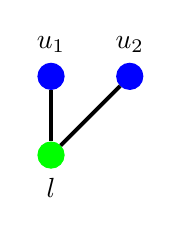
\begin{tikzpicture}
		\node[shape=circle,draw=blue,fill=blue,label=above:$u_1$] (u1) {};
		\node[shape=circle,draw=blue,fill=blue,label=above:$u_2$] (u2) [right of=u1] {};
		\node[shape=circle,draw=green,fill=green,label=below:$l$] (l) [midway, below of=u1] {};

		\draw (u1) [line width=0.5mm] -- (l);
		\draw (u2) [line width=0.5mm] -- (l);
		\end{tikzpicture}
	\caption{Wedge}
	\label{fig:wedge-example}
\end{subfigure}
\begin{subfigure}[b]{0.3\textwidth}
	\centering
 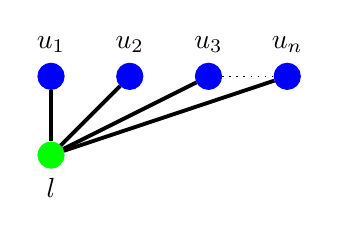
\begin{tikzpicture}
	\node[shape=circle,draw=blue,fill=blue,label=above:$u_1$] (u1) {};
	\node[shape=circle,draw=blue,fill=blue,label=above:$u_2$] (u2) [right of=u1] {};
	\node[shape=circle,draw=blue,fill=blue,label=above:$u_3$] (u3) [right of=u2] {};
	\node[shape=circle,draw=blue,fill=blue,label=above:$u_n$] (un) [right of=u3] {};
	\node[shape=circle,draw=green,fill=green,label=below:$l$] (l) [midway, below of=u2] {};

	\draw (u1) [line width=0.5mm] -- (l);
	\draw (u2) [line width=0.5mm] -- (l);
	\draw (u3) [line width=0.5mm] -- (l);
	\draw (un) [line width=0.5mm] -- (l);
	\draw (u3) [dotted,line width=0.2mm] -- (un);
	\end{tikzpicture}
\caption{Aggregated Wedge}
\label{fig:agg-wedge-example}
\end{subfigure}
\begin{subfigure}[b]{0.3\textwidth}
	\centering
 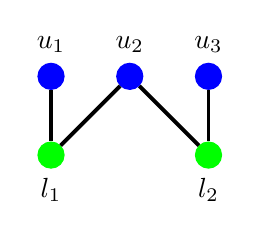
\begin{tikzpicture}
	\node[shape=circle,draw=blue,fill=blue,label=above:$u_1$] (u1) {};
	\node[shape=circle,draw=blue,fill=blue,label=above:$u_2$] (u2) [right of=u1] {};
	\node[shape=circle,draw=blue,fill=blue,label=above:$u_3$] (u3) [right of=u2] {};
	\node[shape=circle,draw=green,fill=green,label=below:$l_1$] (l1) [below of=u1] {};
	\node[shape=circle,draw=green,fill=green,label=below:$l_2$] (l2) [below of=u3] {};

	\draw (u1) [line width=0.5mm] -- (l1);
	\draw (u2) [line width=0.5mm] -- (l1);
	\draw (u2) [line width=0.5mm] -- (l2);
	\draw (u3) [line width=0.5mm] -- (l2);
\end{tikzpicture}
\caption{Double Wedge}
\label{fig:double-wedge-example}
\end{subfigure}
\end{figure}

 
\begin{figure}[htp!]
		\centering
	\tikzsetnextfilename{basic_def_1}
 \begin{tikzpicture}
	\node[shape=circle,draw=blue,fill=blue,label=above:$u_{i1}$] (ui1) {};
	\node[shape=circle,draw=blue,fill=blue,label=above:$u_{i2}$] (ui2) [right of=ui1] {};
	\node[shape=circle,draw=blue,fill=blue,label=above:$u_{in}$] (uin) [right of=ui2] {};
	\node[shape=circle,draw=blue,fill=blue,label=above:$u_{j1}$] (uj1) [right of=uin] {};
	\node[shape=circle,draw=blue,fill=blue,label=above:$u_{j2}$] (uj2) [right of=uj1] {};
	\node[shape=circle,draw=blue,fill=blue,label=above:$u_{jn}$] (ujn) [right of=uj2] {};
	\node[shape=circle,draw=blue,fill=blue,label=above:$u_{k1}$] (uk1) [right of=ujn] {};
	\node[shape=circle,draw=blue,fill=blue,label=above:$u_{k2}$] (uk2) [right of=uk1] {};
	\node[shape=circle,draw=blue,fill=blue,label=above:$u_{kn}$] (ukn) [right of=uk2] {};
	\node[shape=circle,draw=green,fill=green,label=below:$l_1$] (l1) [below of=uin] {};
	\node[shape=circle,draw=green,fill=green,label=below:$l_2$] (l2) [below of=ujn] {};
	\node[draw=black,fit=(ui1) (ui2) (uin)] {};
	\node[draw=black!60!green,fit=(uj1) (uj2) (ujn)] {};
	\node[draw=black!30,fit=(uk1) (uk2) (ukn)] {};
	\draw (ui1) [line width=0.5mm] -- (l1);
	\draw (ui2) [line width=0.5mm] -- (l1);
	\draw (uin) [line width=0.5mm] -- (l1);
	\draw (ui2) [dotted,line width=0.2mm] -- (uin);
	\draw (uj1) [line width=0.5mm] -- (l1);
	\draw (uj2) [line width=0.5mm] -- (l1);
	\draw (ujn) [line width=0.5mm] -- (l1);
	\draw (uj1) [line width=0.5mm] -- (l2);
	\draw (uj2) [line width=0.5mm] -- (l2);
	\draw (ujn) [line width=0.5mm] -- (l2);
	\draw (uj2) [dotted,line width=0.2mm] -- (ujn);
	\draw (uk1) [line width=0.5mm] -- (l2);
	\draw (uk2) [line width=0.5mm] -- (l2);
	\draw (ukn) [line width=0.5mm] -- (l2);
	\draw (uk2) [dotted,line width=0.2mm] -- (ukn);
\end{tikzpicture}
\caption{Aggregated double-wedge}
\label{fig:agg-double-wedge-example}
\end{figure}

 
\begin{figure}[htp!]
\begin{subfigure}[b]{1\textwidth}
	\centering
 \begin{tikzpicture}
	\node[shape=circle,draw=blue,fill=blue,label=above:$u_{i1}$] (ui1) {};
	\node[shape=circle,draw=blue,fill=blue,label=above:$u_{i2}$] (ui2) [right of=ui1] {};
	\node[shape=circle,draw=blue,fill=blue,label=above:$u_{in}$] (uin) [right of=ui2] {};
	\node[shape=circle,draw=blue,fill=blue,label=above:$u_{j1}$] (uj1) [right of=uin] {};
	\node[shape=circle,draw=blue,fill=blue,label=above:$u_{j2}$] (uj2) [right of=uj1] {};
	\node[shape=circle,draw=blue,fill=blue,label=above:$u_{jn}$] (ujn) [right of=uj2] {};
	\node[shape=circle,draw=blue,fill=blue,label=above:$u_{k1}$] (uk1) [right of=ujn] {};
	\node[shape=circle,draw=blue,fill=blue,label=above:$u_{k2}$] (uk2) [right of=uk1] {};
	\node[shape=circle,draw=blue,fill=blue,label=above:$u_{kn}$] (ukn) [right of=uk2] {};
	\node[shape=circle,draw=green,fill=green,label=below:$l_1$] (l1) [below of=ui2] {};
	\node[shape=circle,draw=green,fill=green,label=below:$l_2$] (l2) [below of=uj2] {};
	\node[shape=circle,draw=green,fill=green,label=below:$l_3$] (l3) [below of=uk2] {};
	\node[draw=black,fit=(ui1) (ui2) (uin)] {};
	\node[draw=black!60!green,fit=(uj1) (uj2) (ujn)] {};
	\node[draw=black!30,fit=(uk1) (uk2) (ukn)] {};
	\draw (ui1) [line width=0.5mm] -- (l1);
	\draw (ui2) [line width=0.5mm] -- (l1);
	\draw (uin) [line width=0.5mm] -- (l1);
	\draw (ui1) [line width=0.5mm] -- (l2);
	\draw (uin) [line width=0.5mm] -- (l2);
	\draw (ui2) [dotted,line width=0.2mm] -- (uin);
	\draw (uj1) [line width=0.5mm] -- (l1);
	\draw (uj2) [line width=0.5mm] -- (l1);
	\draw (ujn) [line width=0.5mm] -- (l1);
	\draw (uj1) [line width=0.5mm] -- (l3);
	\draw (uj2) [line width=0.5mm] -- (l3);
	\draw (ujn) [line width=0.5mm] -- (l3);
	\draw (uj2) [dotted,line width=0.2mm] -- (ujn);
	\draw (uk1) [line width=0.5mm] -- (l3);
	\draw (uk2) [line width=0.5mm] -- (l3);
	\draw (ukn) [line width=0.5mm] -- (l3);
	\draw (uk2) [line width=0.5mm] -- (l2);
	\draw (ukn) [line width=0.5mm] -- (l2);
	\draw (uk2) [dotted,line width=0.2mm] -- (ukn);
\end{tikzpicture}
\caption{Aggregated bi-triangle}
\label{fig:agg-bt-example}
\end{subfigure}
\end{figure}

 

\begin{table}[!ht]
\centering
\begin{tabular}{|c|l|} \hline
\textbf{Notation} & \textbf{Meaning}\\ \hline
$G=((U\cup L),E)$ & a bipartite graph\\  \hline
$n,m$ & the number of vertices and edges in $G$, resp.\\  \hline
$(u,l)$ & an edge between vertices $u$ and $l$\\  \hline
$\bti$ & the bi-triangle $u_1,l_1,u_2,l_3,u_3,l_2,u_1$\\  \hline
$\bt$ & the set of all the possible bi-triangles in $G$ \\  \hline
$bt$ & Subset of $\bt$, such that $bt \subseteq \bt$ \\  \hline
$\at$ & the set of all the possible Aggregated bi-triangles in $G$ \\  \hline
$at$ & Subset of $\at$, such that $at \subseteq \at$ \\  \hline
$(u_1,l,u_2)$ & a wedge with  middle vertex $l$\\  \hline
$\la l, W_l \ra$ & an aggregated wedge\\  \hline
$\aw$ & the set of all the possible aggregated wedges in $G$\\  \hline
$aw$ & Subset of $\aw$, such that $aw \subseteq \aw$ \\  \hline
$(u_1,l_1,u_2,l_2,u_3)$ & a double wedge with middle vertices $l_1$ and $l_2$\\  \hline 
$\dw$ & the set of all the possible double-wedges in $G$\\  \hline
$dw$ & Subset of $\dw$, such that $dw \subseteq \dw$ \\  \hline
$\la (l_1, l_2), U_t \ra$ & an aggregated double wedge\\  \hline
$\la (l_1, l_2,l_3), \hat{U}_t \ra$ & an aggregated bi-triangle\\  \hline
\end{tabular}
\caption{Summary of notations and their meanings.}
\label{table:notation}
\end{table}
      

\subsection{Algorithm Sketch}
Dynamic Pipeline Algorithm for Enumerating Bi-triangles ($\dpbt$) is defined in terms of the behavior of its four kinds stages: \textit{Source} ($\ibt$),  
\textit{Generator} ($\gbt$),  \textit{Sink} ($\obt$), and \textit{Filter}($\fbt$) stages. The algorithm tries to collect all the previous object definitions 
(\acrshort{awg}, \acrshort{adwg} and \acrshort{abt}) during the execution of the actors of $\fbt$ instance. Since we are dealing with different object representations,
the following channels are connecting the stages in $\dpbt$.

\begin{table}[ht]
\centering
\begin{tabular}{|p{0.2\linewidth}|p{0.8\linewidth}|} \hline
\textbf{Channel} & \textbf{Meaning}\\ \hline
$IC$ & Set of Input Channels \\ \hline
$OC$ & Set of Output Channels \\ \hline
$IC_E$ & Input Channels carrying $e \in E$ \\ \hline
$OC_E$ & Output Channels carrying $e \in E$ \\ \hline
$IC_{W_1}$ & Input Channels carrying \acrshort{awg} \\ \hline
$OC_{W_1}$ & Output Channels carrying \acrshort{awg} \\ \hline
$IC_{W_2}$ & Input Channels carrying \acrshort{awg}, second round \\ \hline
$OC_{W_2}$ & Output Channels carrying \acrshort{awg}, second round \\ \hline
$IC_Q$ & Input Channels carrying $Q$ Command \\ \hline
$OC_Q$ & Output Channels carrying $Q$ Command \\ \hline
$IC_{BT}$ & Input Channels carrying $\bt$ \\ \hline
$OC_{BT}$ & Output Channels carrying $\bt$ \\ \hline
\end{tabular}
\caption{Summary of Channels used in DP}
\label{table:channels}
\end{table}

\begin{definition}[Filter State]
Let $G=((U\cup L),E)$ be a bipartite graph. 
Let $\aw$ be a set of all possibles Aggregated wedges in $G$.
Let $\dw$ be a set of all possibles Aggregated double-wedges in $G$.
Let $\at$ be a set of all possibles Aggregated bi-triangles in $G$.
An \textit{filter state} of DP is a sum type $\st = aw + dw + at$, such that $aw \subseteq \aw, dw \subseteq \dw, at \subseteq \at$.
\end{definition}
 
\paragraph{Sketch} $\ibt$ reads from some input stream all $(u,l) \in E$ in an incremental non-blocking manner and transfer to the following stage each $(u,l)$ using $OC_E$.
For every $(u,l)$ that arrives to $\gbt$, a new $\fbt$ instance with parameter $l \in L$ is spawn. $\fbt$ contains four actors. These four functions builds incrementally all the object definitions exposed before. 
First \mintinline{shell}{actor1} will received from $IC_E$ all the rest of the edges of the original $G$ and tries to build \acrshort{awg} and downstream to $\fbt$ using $OC_{W1}$. 
Then \mintinline{shell}{actor2} receives from $IC_{W1}$ aggregated wedges from previous $\fbt$, downstream to next $\fbt$ and $\gbt$ using $OC_{W1}$ and at the same time use its information to see 
if it can build \acrshort{adwg}. If it can, it will store in its $\st$ those $dw \in \dw$.

In \mintinline{shell}{actor2} we have exposed that it downstream the \acrshort{awg} to  $\fbt$ and $\gbt$. This is because we need to retro feed all the pipeline with all the \acrshort{awg}, in order to find 
possible wedges for each $\fbt$ that connects some \acrshort{dwg}. Remember that by definition a \acrshort{bt} is a \acrshort{dwg} connected to a \acrshort{wg} in a cycle, with a particular disposition of the edges.
Having said that, \mintinline{shell}{actor3} receives all the \acrshort{awg} again but in a different channel $IC_{W2}$ and builds \acrshort{abt} and store them in $\st$. If there is a match, 
\mintinline{shell}{actor4} will enumerate those \acrshort{bt} extracted from $\st$ and downstream to $\obt$ through $OC_{BT}$.

\subsection{Dynamic Pipeline for Enumerating Bi-triangles}

%      
\begin{table}[ht]
\centering
\begin{tabular}{|p{0.3\linewidth}|p{0.7\linewidth}|} \hline
\textbf{Function} & \textbf{Meaning}\\ \hline
$\sw(F,l,\st)$ & Spawn new filter instance with parameters $F$ (Filter template), $l \in L$ and $\st$ as the State of the Filter\\\hline
$\fd$ & Kill this filter instance because PostCondition does not fullfil\\ \hline
$\fid$ & State after calling $\fd$ on filter. Indicates if Filter is die or not. If it is died, this filter instance does not participate anymore in the pipeline streaming processor\\ \hline
$\gs$ & Get Current State $\st$ for Filter Instance \\ \hline
$\us(\st)$ & Update Current State $\st$ for Filter Instance \\ \hline
$\p(\mathtt{v}, OC_x)$ & push some value $\mathtt{v}$ to some Output Channel $OC_x$ \\\hline
$\mt(Q, BT)$ & Check if a Query $Q$ matches over $BT$ \\ \hline
\end{tabular}
\caption{Summary of auxiliary functions for handling DP internals.}
\label{table:aux:fn}
\end{table}
%      
%
%      
      
\begin{algorithm}
\SetKwInOut{P}{Input Data}
\SetKwInOut{Q}{Input Commands}
\SetKwInOut{IC}{Input Channels}
\SetKwInOut{OC}{Output Channels}
\SetAlgorithmName{Source}{src}{}
\SetAlgoRefName{$S_r$}
\P{$IO_E$: File or Input Stream with Set of Edges $E$}
\Q{$IO_Q$: File or Input Stream with Commands $Q$}
\IC{$IC = \la IC_{W_2} \ra$}
\OC{$OC = \la OC_E, OC_{W_2}, OC_Q \ra$}
\ForAll(\tcp*[f]{Edges to Generator/Filter}){$(u,l) \in IO_E$}
{$\p((u,l), OC_E)$
}
\ForAll(\tcp*[f]{Feedback from Generator to Filter}){$\la l, W_l \ra \in IC_{W_2}$}
{$\p(\la l, W_l \ra, OC_{W_2})$
}
\ForAll(\tcp*[f]{Send Query Commands}){$Q \in IO_Q$}
{$\p(Q, OC_Q)$
}
\caption{This is the algorithm of the DP Source}
\end{algorithm}

\begin{algorithm}
\SetKwInOut{P}{Filter Template}
\SetKwInOut{IC}{Input Channels}
\SetKwInOut{OC}{Output Channels}
\SetAlgorithmName{Generator}{gen}{}
\SetAlgoRefName{$G$}
\P{$F$}
\IC{$ IC = \la IC_E, IC_{W_1}, IC_Q, IC_{BT} \ra$}
\OC{$ OC = \la OC_{W_2}, OC_{BT} \ra$}
\ForAll{$(u,l) \in IC_E$}
{$\sw(F, l, \la l, \{u\} \ra)$
}
\ForAll(\tcp*[f]{Feedback channel to retrofit Source}){$\la l, W_l \ra \in IC_{W_1}$}
{$\p(\la l, W_l \ra, OC_{W_2})$
}
\ForAll{$\bti \in IC_{BT}$}
{$\p(\bti, OC_{BT})$
}
\caption{This is the algorithm of the DP Generator}
\end{algorithm}

\begin{algorithm}
\SetKwInOut{IC}{Input Channels}
\SetKwInOut{O}{Output}
\SetAlgorithmName{Sink}{sink}{}
\SetAlgoRefName{$S_k$}
\O{$IO_{BT}$: File or Output Stream with $BT$}
\IC{$IC = \la IC_{BT} \ra$}
\ForAll(\tcp*[f]{Read Results and put in $IO_{BT}$}){$\bti \in IC_{BT}$}
{$put(\bti, IO_{BT})$
}
\caption{This is the algorithm of the DP Sink}
\end{algorithm}

\begin{algorithm}
\SetKwInOut{P}{Parameter}
\SetKwInOut{IC}{Input Channels}
\SetKwInOut{OC}{Output Channels}
\SetKwInOut{FS}{$\st$}
\SetKwInOut{PC}{Post-Cond}
\SetKwInOut{PrC}{Pre-Cond}
\SetKwFunction{aa}{actor1}
\SetKwProg{df}{def}{:}{end}
\SetAlgorithmName{Filter}{fa1}{}
\SetAlgoRefName{actor1}
\P{$l \in L$}
\FS{$\la l, W_l \ra$}
\IC{$ IC = \la IC_E, IC_{W_1}, IC_{W_2}, IC_Q, IC_{BT} \ra $}
\OC{$ OC = \la OC_E, OC_{W_1}, OC_{W_2}, OC_Q, OC_{BT} \ra $}
\PC{$|W_l| > 1 \lor \fid$}
\BlankLine
\df{\aa{}}{
$\la l, W_l \ra \leftarrow \gs$\\
\ForAll{$(u',l') \in IC_E$}
{\uIf{$l = l'$}{$W_l \leftarrow W_l \cup \{u'\}$}
}
\uIf{$|W_l| > 1$}{
      $\us(\la l, W_l \ra)$\\
      $\p(\la l, W_l \ra, OC_{W_1})$\\
}\Else{$\fd$}
}
\caption{This actor tries to build a Set of vertices $W_l \subseteq U$ adjancents to $l$ Filter parameter }
\end{algorithm}

\begin{algorithm}
\SetKwInOut{P}{Parameter}
\SetKwInOut{IC}{Input Channels}
\SetKwInOut{OC}{Output Channels}
\SetKwInOut{FS}{$\st$}
\SetKwInOut{PC}{Post-Cond}
\SetKwInOut{PrC}{Pre-Cond}
\SetKwFunction{ab}{actor2}
\SetKwProg{df}{def}{:}{end}
\SetAlgorithmName{Filter}{fa2}{}
\SetAlgoRefName{actor2}
\P{$l \in L$}
\FS{$\la l, W_l \ra$}
\IC{$ IC = \la IC_E, IC_{W_1}, IC_{W_2}, IC_Q, IC_{BT} \ra $}
\OC{$ OC = \la OC_E, OC_{W_1}, OC_{W_2}, OC_Q, OC_{BT} \ra $}
\BlankLine
\PrC{$W_l \subseteq U, |W_l| > 1$}
\PC{$dw \subseteq \dw, |dw| \geq 1 \lor \fid$}
\df{\ab{}}{
$\la l, W_l \ra \leftarrow \gs$\\
\ForAll{$\la l', W_l' \ra \in IC_{W_1}$}{
      \tcp*[h]{By pass Wedges from previous filters to next ones}
      $\p(\la l', W_l \ra, OC_{W_1})$\\
      $dw \leftarrow \emptyset$\\
      \If{$l \neq l' \land W_l' \cap W_l \neq \emptyset$}{
            $(l_l, l_u) \leftarrow (\argmin_{l,l'}, \argmax_{l,l'})$\\
            \uIf{$l < l'$}{
                  $(W_{l_l}, W_{l_u}) \leftarrow (W_l, W_l')$
            }\Else{
                  $(W_{l_l}, W_{l_u}) \leftarrow (W_l', W_l)$
            }
            $I \leftarrow W_{l_l} \setminus W_{l_u}$\\
            $J \leftarrow W_{l_l} \cap W_{l_u}$\\
            $K \leftarrow W_{l_u} \setminus W_{l_l}$\\
            $dw \leftarrow dw \cup \{\la (l, l'), \la I, J, K\ra \ra\}$
      }
}
\uIf{$dw = \emptyset$}{$\fd$}
\Else{$\us(dw)$}
}
\caption{This actor tries to build a Set of all possible Aggregated double-wedges $dw = \{\la (l,l'), U_t \ra\}, dw \subseteq \dw$, which first component $l$ is the Parameter of the Filter}
\end{algorithm}

\begin{algorithm}
\DontPrintSemicolon
\SetKwInOut{P}{Parameter}
\SetKwInOut{IC}{Input Channels}
\SetKwInOut{OC}{Output Channels}
\SetKwInOut{FS}{$\st$}
\SetKwInOut{PC}{Post-Cond}
\SetKwInOut{PrC}{Pre-Cond}
\SetKwFunction{ac}{actor3}
\SetKwProg{df}{def}{:}{end}
\SetAlgorithmName{Filter}{fa3}{}
\SetAlgoRefName{actor3}
\P{$l \in L$}
\FS{$dw \subseteq \dw$}
\IC{$ IC = \la IC_E, IC_{W_1}, IC_{W_2}, IC_Q, IC_{BT} \ra $}
\OC{$ OC = \la OC_E, OC_{W_1}, OC_{W_2}, OC_Q, OC_{BT} \ra $}  
\BlankLine
\PrC{$dw \subseteq \dw, |dw| \geq 1$}
\PC{$at \subseteq \at, |at| \geq 1 \lor \fid$}
\df{\ac{}}{
      $dw \leftarrow \gs$\\
      \ForAll{$\la l', W_l' \ra \in IC_{W_2}$}{
            \tcp*[h]{By pass to be used by following Filters}
            $\p(\la l', W_l' \ra, OC_{W_2})$\\ 
            \tcp*[h]{For each double wedge in State}\\
            \ForEach{$\la (l_l, l_u), \la I, J, K \ra \ra \in dw, l_l < l' \land l_u > l'$}{
                  $I' \leftarrow I \cup J$\\
                  $K' \leftarrow K \cup J$\\
                  \If{$W_l' \cap I' \neq \emptyset \land W_l' \cap K' \neq \emptyset$}{
                        $I' \leftarrow I' \cap W_l'$\\
                        $K' \leftarrow K' \cap W_l'$\\
                        $U_t' \leftarrow U_t' \cup \{\la I', J, K' \ra\})$
                  }
                  \If{$U_t' \neq \la \emptyset,\emptyset,\emptyset \ra$}{
                        $at \leftarrow at \cup \{\la (l_l, l', l_u), U_t' \ra\}$
                  }
            }
      }
      \uIf{$at = \emptyset$}{$\fd$}
      \Else{$\us(at)$\\}
}
\caption{This actor try to build a Set of all possible Aggregated bi-triangles $\at = \{\la (l_l, l_m, l_u), U_t \ra\}, at \subseteq \at$, , such that $l = l_l \lor l = l_u$, where $l$ is the Filter Parameter}
\end{algorithm}

\begin{algorithm}
\SetKwInOut{P}{Parameter}
\SetKwInOut{IC}{Input Channels}
\SetKwInOut{OC}{Output Channels}
\SetKwInOut{FS}{$\st$}
\SetKwInOut{PC}{Post-Cond}
\SetKwInOut{PrC}{Pre-Cond}
\SetKwFunction{ad}{actor4}
\SetKwFunction{butV}{buildBtVertex}
\SetKwFunction{butE}{buildBtEdge}
\SetKwProg{df}{def}{:}{end}
\SetAlgorithmName{Filter}{fa4}{}
\SetAlgoRefName{actor4}
\P{$l \in L$}
\FS{$at \subseteq \at$}
\IC{$ IC = \la IC_E, IC_{W_1}, IC_{W_2}, IC_Q, IC_{BT} \ra $}
\OC{$ OC = \la OC_E, OC_{W_1}, OC_{W_2}, OC_Q, OC_{BT} \ra $}  
\BlankLine
\PrC{$at \subseteq \at, |at| \geq 1$}
\df{\ad{}}{
$at \leftarrow \gs$\\
\ForAll{$Q \in IC_Q$}{
      \ForEach{$\la (l_l, l_m, l_u), \la I,J,K \ra \ra \in at$}{
            \Switch{$Q$}{
                  \Case{$Q_V$}{
                        \If{$Q_V \cap \{l_l, l_m, l_u\} \neq \emptyset \lor Q_V \cap (I \cup J \cup K) \neq \emptyset$}{
                              $bt \leftarrow \butV(\la (l_l, l_m, l_u), \la I,J,K \ra \ra), Q_V)$\\
                              \ForAll{$\bti \in bt$}{
                                    $\p(\bti, OC_{BT})$
                              }
                        }
                  }
                  \Case{$Q_E$}{
                        \ForEach{$(u,l) \in Q_E$}{
                              \If{$(l = l_l \lor l = l_m \lor l = l_u) \land u \in (I \cup J \cup K)$}{
                                    $bt \leftarrow \butE(\la (l_l, l_m, l_u), \la I,J,K \ra \ra), (u,l))$\\
                                    \ForAll{$\bti \in bt$}{
                                          $\p(\bti, OC_{BT})$
                                    }
                              }
                        }
                  }
            }
      }
}
}
\caption{This actor tries to process Query Commands $Q$ that arrives through Channel $IC_Q$. If they match with some Bi-triangles that are contained in this Filter, it will pass to the result Channel $OC_{BT}$ to be processed by the Sink}
\end{algorithm}


\begin{algorithm}
\SetKwInOut{I}{Input}
\SetKwInOut{O}{Output}
\SetKwFunction{but}{buildBtVertex}
\SetKwProg{df}{def}{:}{end}
\SetAlgorithmName{Function}{a1}{}
\SetAlgoRefName{buildBtVertex}
\I{$\la (l_l, l_m, l_u), \la I,J,K \ra \ra \in at, at \subseteq \at$}
\I{$Q_V$}
\O{$bt \subseteq \bt$ or $\emptyset$ if cannot build any $bt$}
\df{\but{$\la (l_l, l_m, l_u), \la I,J,K \ra \ra$, $Q_V$}}{
      $bt \leftarrow \emptyset$\\
      \uIf{$Q_V \cap \{l_l, l_m, l_u\}$}{
            \tcp*[h]{If it is in lower i need to build all for this lower triplet}\\
            \ForEach{$i \in I$}{
                  \ForEach{$j \in J, j \neq i$}{
                        \ForEach{$k \in K, k \neq i \land k \neq j$}{
                              $bt \leftarrow bt \cup \{BT_{(l_l, l_m,l_u)}^{(i, j, k)}\}$
                        }
                  }
            }
      }\Else{
            \tcp*[h]{Otherwise just build those that are in the this upper $v$}\\
            \ForEach{$i \in I$}{
                  \ForEach{$j \in J, j \neq i$}{
                        \ForEach{$k \in K, k \neq i \land k \neq j \land (Q_V \cap \{i,j,k\} \neq \emptyset$}{
                              $bt \leftarrow bt \cup \{BT_{(l_l, l_m,l_u)}^{(i, j, k)}\}$
                        }
                  }
            }
      }
      \Return{$bt$}
}
\caption{Given a Set of Vertex Try to build the set of all possible bi-triangles based on Aggregated bi-triangles information in $\la (l_l, l_m, l_u), \la I,J,K \ra \ra \in at, at \subseteq \at$ param}
\end{algorithm}

\begin{algorithm}
\SetKwInOut{I}{Input}
\SetKwInOut{O}{Output}
\SetKwFunction{but}{buildBtEdge}
\SetKwFunction{he}{hasEdge}
\SetKwProg{df}{def}{:}{end}
\SetAlgorithmName{Function}{a2}{}
\SetAlgoRefName{buildBtEdge}
\I{$\la (l_l, l_m, l_u), \la I,J,K \ra \ra \in at, at \subseteq \at$}
\I{$(u,l)$}
\O{$bt \subseteq \bt$ or $\emptyset$ if cannot build any $bt$}
\df{\but{$\la (l_l, l_m, l_u), \la I,J,K \ra \ra$, $Q_V$}}{
      $bt \leftarrow \emptyset$\\
      \ForEach{$i \in I$}{
            \ForEach{$j \in J, j \neq i$}{
                  \ForEach{$k \in K, k \neq i \land k \neq j \land \he((u,l), (l_l,l_m,l_u),(i,j,k))$}{
                        $bt \leftarrow bt \cup \{BT_{(l_l, l_m,l_u)}^{(i, j, k)}\}$
                  }
            }
      }
      \Return{$bt$}
}
\df{\he{$(u,l), (l_l,l_m,l_u), (i,j,k)$}}{
      \If{$(u,l) = (l_l, i) \lor (u,l) = (l_l, j) \lor (u,l) = (l_u, j) \lor (u,l) = (l_u, k) \lor (u,l) = (l_m, i) \lor (u,l) = (l_m, k)$}{
            \Return{True}
      }\Else{
            \Return{False}
      }
}
\caption{Given a Set of Edges Try to build the set of all possible bi-triangles based on Aggregated bi-triangles information in $\la (l_l, l_m, l_u), \la I,J,K \ra \ra \in at, at \subseteq \at$ param}
\end{algorithm}
      
\clearpage
\section{Draft-Correctness of the Algorithm}

A bi-triangle can be described as a sequence $(a,A,b,B,c,C)$  where $\{ a,b,c\} \in L$  and $\{ A,B,C\} \in U\footnote{In the enumeration, L and $U$ be interchanged}$

We need to prove that the algorithm can enumerate all   bi-triangle in the graph and also that there are not duplicates in the enumeration.

\begin{quote}
Very recently, Qiao
et al. proposed CrystalJoin [41] that aims at resolving the
output crisis by compressing the (intermediate) results (taken from Distributed Subgraph Matching on Timely Dataflow).
\end{quote}

We use the same technique, compressing a group of bi-triangles as $(a,b,c,(I,J,K))$. 
\begin{definition}{Compress representation of bi-triangles}

$(a,b,c,(I,J,K))$  where  $I, J,K$ are sets of upper nodes. $I$ is the set of nodes  incident to $a$ and $b$, $J$ is the set of nodes incident to $a$ and $c$ and $K$ is the set of nodes incident to $b$ and $c$.
\end{definition}
\begin{algorithm}{Listing bi-tringles}

Listing bi-tringles, from this compressed representation, stands for finding  triples $(A,B,C)$ such that $A \in I$, $B \in J$  and $C \in K$, all pairwise distinct.
\end{algorithm} 

First we are going to prove that if we take all the triples $(a,b,c)$  such $a<b$ and $b<c$  and    $(a,A,b,B,c,C)$ is a bi-triangle, then it is not listed twice (theorem \ref{TH-unicity}).  We will show that we  enumerate all the bi-triangles  where $A,B,C$  are distinct and $A$ is incident to $a$ and $b$, $B$is incident to $a$ and $c$ and $C$ is incident to $b$ and $C$ (theorem \ref{TH-all}). 
\begin{theorem} \label{TH-unicity}Every bi-triangle is listed at most once 

\end{theorem}
\begin{proof}
As a bi-triangle is a 6-closed cycle it can be described as a sequence of nodes  $(a,A,b,B,c,C)$, each one adjacent to its neighbour. For every feasible permutation  starting with a node in $L$ we are going to proof that only one will be accepted by actor3.  
\begin{itemize}
    \item $(b,C,c,B,a,A)$ not accepted because $c > a$
    \item $(b,A,a,B,c,C)$ not accepted because $b > a$
    \item $(c,B,a,A,b,C)$ not accepted because $c > a$ and $c > b$
    \item $(c,C,b,A,a,B)$ not accepted because $c > a  $
    \item $(a,A,b,C,c,B)$ is accepted because $a < c $ in actor 2 of filter $F_a$ or $F_c$ and $a < b <c$  in actor 3
    \item $(a,B,c,C,b,A)$ not accepted because $c > a$
\end{itemize}


Therefore the  only sequence constructed by the algorithm is the one that satisfies $a < b < c $ where $A,B,C$  are distinct and $A$ is incident to $a$ and $b$, $B$ is incident to $a$ and $c$ and $C$ is incident to $b$ and $C$.
\end{proof}


\begin{theorem}\label{TH-all}Every bi-triangle present in the graph is listed.

\end{theorem}

\begin{proof}

Obvious  from the definition of $I,J,K$  and the algorithm of obtaining bi-triangles. 
\iffalse
Lets assume that a bi-triangle $(a,A,b,B,c,C)$   will assume that $a$ is the smallest element in the set $\{a,b,c\}$ and $c$ is the bigger.
When actor 1 in fiter $F_a$1 ends reading all the edges, $\{A,B\} \subseteq W_a$. Also When actor 1 in fiter $F_c$1 ends reading all the edges, $\{B,C\} \subseteq W_c$. 

AS $a < c$  in filter $F_a$ the pair $(a,c)$  will be added to D
$DW$. When actor 3 in filter $F_a$ receives $(b, W_b)$ will add to $BT$ because of the non empty intersection. Therefore the bi-triangle $(a,A,b,B,c,C)$ can be recognized
\fi
\end{proof}
\iffalse So we are going to talk from now on of the bi-triangles produced by the filter $F_a$ or by the filter $F_c$.

 At the end of the execution of actor 3 $F_a$ constructs the sets where to choose $A,B,C$
 
 Actor 1 collects in $F_a$ all the nodes in $U$ adjacent to $a$ i.e. all the candidates to choose $A$. Afterwards this set will be reduced . 
 
 Actor 2 receives pairs $(c,V)$ where $V$ are all the nodes adjacent to $c$. It adds the set of nodes $c$ if $c>a+1$ collecting all the nodes adjacent to each $c$, constructing 3 sets of nodes belonging to $U$.
 
 Actor 3 receives pairs $(b,M) $ where $M$ are all the nodes adjacent to $b$
 
 Actor3 accepts b as a candidate if
 
 \begin{enumerate}
     \item $a < b < c$
 \end{enumerate}
 
 the only thing to prove is:
 
 \begin{enumerate}
     \item bi triangles satisfying $a < b < c$ are listed once
     \item bi triangles satisfying $a < c < b$ are also listed and only  once
 \end{enumerate}
 
 the bi-triangle  $(a,A,b,B,c,C)$ can be listed as 
 
 \begin{enumerate}
     \item $(,,,,,)$
      \item $(,,,,,)$
       \item $(,,,,,)$
        \item $(,,,,,)$
         \item $(,,,,,)$
          \item $(,,,,,)$
 \end{enumerate}
 
 All the configurations are rejected by filters $F_b$ and $F_c$, and the listing starting with $a$ the ordered one is accepted and the unordered rejected  \fi
 
 \section{Implementation using \acrshort{dpf} in \acrshort{hs}}

 \section{Chapter Summary}